\section{Raw Data}

% \begin{table}[H]
%     \centering
%     \label{tab:common:table:jni}
%     \caption{Common table for JNI tests, Time(ns)}
%     \resizebox{\columnwidth}{!}{
%         \begin{tabular}{|l|c|c|c|}\hline
\textbf{Block size}  & \textbf{Benchmark convert param to vector} & \textbf{Benchmark with no params} & \textbf{Benchmark with vector as param}\\\hline
\textbf{16}  & 5946.0667 $\pm$ 784.3565 & 2557.1667 $\pm$ 493.7816 & 2979.2333 $\pm$ 96.2158\\\hline
\textbf{32}  & 5600.7333 $\pm$ 191.3485 & 2251.7333 $\pm$ 18.0875 & 2953.1000 $\pm$ 24.5474\\\hline
\textbf{64}  & 5789.9333 $\pm$ 316.5874 & 2274.4000 $\pm$ 20.3493 & 2939.2667 $\pm$ 20.0347\\\hline
\textbf{128}  & 8071.4000 $\pm$ 3161.5874 & 2550.4000 $\pm$ 497.6299 & 3309.0667 $\pm$ 328.8276\\\hline
\textbf{256}  & 7586.8333 $\pm$ 488.9577 & 2295.1667 $\pm$ 22.9024 & 3088.5000 $\pm$ 59.1501\\\hline
\textbf{512}  & 10175.3667 $\pm$ 1575.4113 & 2343.8667 $\pm$ 21.3224 & 3208.3333 $\pm$ 131.3823\\\hline
\textbf{1024}  & 7036.3000 $\pm$ 1666.6088 & 2333.3667 $\pm$ 16.5224 & 4486.2000 $\pm$ 1041.4911\\\hline
\textbf{2048}  & 6954.9333 $\pm$ 976.3683 & 2400.9333 $\pm$ 88.2733 & 3970.4000 $\pm$ 306.6608\\\hline
\textbf{4096}  & 7543.4000 $\pm$ 2469.1806 & 2349.0000 $\pm$ 54.1446 & 4284.7000 $\pm$ 869.9760\\\hline
\textbf{8192}  & 7359.3000 $\pm$ 2058.9155 & 2316.0000 $\pm$ 18.7790 & 3911.4333 $\pm$ 322.5315\\\hline
\textbf{16384}  & 6401.1333 $\pm$ 524.5899 & 2312.4667 $\pm$ 17.3997 & 5355.7333 $\pm$ 631.9348\\\hline
\textbf{32768}  & 10168.4333 $\pm$ 3104.6108 & 2309.0333 $\pm$ 19.1719 & 6260.3000 $\pm$ 1008.9804\\\hline
\textbf{65536} & 12772.4667 $\pm$ 2355.3669 & 1989.6000 $\pm$ 181.0611 & 6064.3333 $\pm$ 675.6516\\\hline
\end{tabular}

%     }
% \end{table}
%
% \begin{table}[H]
%     \centering
%     \label{tab:common:table:cpp}
%     \caption{Common table for C++ tests, Time (ms)}
%     \resizebox{\columnwidth}{!}{
%         \begin{tabular}{|l|c|c|c|c|c|}\hline
\textbf{Block size}  & \textbf{Columbia converted Iterative} & \textbf{Columbia optimized Iterative} & \textbf{KISS} & \textbf{Princeton converted Iterative} & \textbf{Princeton converted Recursive}\\\hline
\textbf{16}  & 0.0225 $\pm$ 0.0033 & 0.0198 $\pm$ 0.0025 & 0.0195 $\pm$ 0.0067 & 0.0342 $\pm$ 0.0053 & 0.0612 $\pm$ 0.0065\\\hline
\textbf{32}  & 0.0322 $\pm$ 0.0025 & 0.0322 $\pm$ 0.0031 & 0.0239 $\pm$ 0.0031 & 0.0545 $\pm$ 0.0043 & 0.1085 $\pm$ 0.0020\\\hline
\textbf{64}  & 0.0525 $\pm$ 0.0014 & 0.0524 $\pm$ 0.0012 & 0.0338 $\pm$ 0.0020 & 0.0847 $\pm$ 0.0059 & 0.2148 $\pm$ 0.0024\\\hline
\textbf{128}  & 0.1025 $\pm$ 0.0033 & 0.0814 $\pm$ 0.0127 & 0.0629 $\pm$ 0.0084 & 0.1328 $\pm$ 0.0029 & 0.4517 $\pm$ 0.0057\\\hline
\textbf{256}  & 0.0925 $\pm$ 0.0178 & 0.0822 $\pm$ 0.0039 & 0.1158 $\pm$ 0.0035 & 0.2807 $\pm$ 0.0073 & 0.9139 $\pm$ 0.0067\\\hline
\textbf{512}  & 0.1709 $\pm$ 0.0267 & 0.1744 $\pm$ 0.0308 & 0.2109 $\pm$ 0.0049 & 0.5486 $\pm$ 0.0253 & 1.9142 $\pm$ 0.0102\\\hline
\textbf{1024}  & 0.3656 $\pm$ 0.0284 & 0.3397 $\pm$ 0.0108 & 0.4072 $\pm$ 0.0086 & 1.1691 $\pm$ 0.0172 & 4.0665 $\pm$ 0.0127\\\hline
\textbf{2048}  & 0.9177 $\pm$ 0.0541 & 0.7402 $\pm$ 0.0190 & 0.8635 $\pm$ 0.0243 & 2.4714 $\pm$ 0.0188 & 8.7235 $\pm$ 0.0725\\\hline
\textbf{4096}  & 1.6737 $\pm$ 0.0461 & 1.9889 $\pm$ 0.0982 & 1.9558 $\pm$ 0.1347 & 5.3867 $\pm$ 0.1000 & 18.3487 $\pm$ 0.1235\\\hline
\textbf{8192}  & 3.7768 $\pm$ 0.1838 & 3.8584 $\pm$ 0.2236 & 3.8499 $\pm$ 0.1603 & 11.7050 $\pm$ 0.5076 & 38.4780 $\pm$ 0.6441\\\hline
\textbf{16384}  & 8.2947 $\pm$ 0.3759 & 8.5556 $\pm$ 0.5672 & 7.8854 $\pm$ 0.2775 & 24.3807 $\pm$ 0.5902 & 80.4920 $\pm$ 0.8228\\\hline
\textbf{32768}  & 19.1886 $\pm$ 1.1809 & 18.5907 $\pm$ 0.9959 & 17.6197 $\pm$ 0.5490 & 52.3713 $\pm$ 1.1313 & 167.3867 $\pm$ 1.5300\\\hline
\textbf{65536} & 42.8520 $\pm$ 1.4120 & 44.2337 $\pm$ 2.4361 & 38.3601 $\pm$ 0.7332 & 112.4273 $\pm$ 1.1197 & 346.7600 $\pm$ 1.9190\\\hline
\end{tabular}

%     }
% \end{table}
%
% \begin{table}[H]
%     \centering
%     \label{tab:common:table:java}
%     \caption{Common table for Java tests, Time (ms)}
%     \resizebox{\columnwidth}{!}{
%         \begin{tabular}{|l|c|c|c|}\hline
\textbf{Block size}  & \textbf{Columbia Iterative} & \textbf{Princeton Iterative} & \textbf{Princeton Recursive}\\\hline
\textbf{16}  & 0.0210 $\pm$ 0.0008 & 0.1738 $\pm$ 0.0368 & 0.2730 $\pm$ 0.0708\\\hline
\textbf{32}  & 0.0429 $\pm$ 0.0018 & 0.0571 $\pm$ 0.0071 & 0.3983 $\pm$ 0.0568\\\hline
\textbf{64}  & 0.0906 $\pm$ 0.0010 & 0.0916 $\pm$ 0.0073 & 0.2104 $\pm$ 0.0402\\\hline
\textbf{128}  & 0.2233 $\pm$ 0.0382 & 0.2353 $\pm$ 0.0339 & 0.3204 $\pm$ 0.0425\\\hline
\textbf{256}  & 0.0372 $\pm$ 0.0022 & 0.4380 $\pm$ 0.0316 & 0.7415 $\pm$ 0.0431\\\hline
\textbf{512}  & 0.0754 $\pm$ 0.0029 & 0.9865 $\pm$ 0.0672 & 1.7743 $\pm$ 0.1944\\\hline
\textbf{1024}  & 0.1507 $\pm$ 0.0059 & 2.0255 $\pm$ 0.0933 & 3.5339 $\pm$ 0.2466\\\hline
\textbf{2048}  & 0.4299 $\pm$ 0.0312 & 4.5366 $\pm$ 0.3038 & 8.2740 $\pm$ 0.6905\\\hline
\textbf{4096}  & 0.9984 $\pm$ 0.0915 & 10.6191 $\pm$ 0.8679 & 17.9445 $\pm$ 0.9022\\\hline
\textbf{8192}  & 2.3125 $\pm$ 0.2709 & 27.5617 $\pm$ 1.9755 & 37.6118 $\pm$ 1.5008\\\hline
\textbf{16384}  & 4.8597 $\pm$ 0.4114 & 62.6869 $\pm$ 1.7191 & 80.1848 $\pm$ 1.9414\\\hline
\textbf{32768}  & 11.2535 $\pm$ 0.9718 & 155.5247 $\pm$ 2.7411 & 172.5062 $\pm$ 2.2489\\\hline
\textbf{65536} & 26.3906 $\pm$ 2.1662 & 366.0557 $\pm$ 2.8910 & 366.6833 $\pm$ 3.3610\\\hline
\end{tabular}

%     }
% \end{table}
%
% \begin{table}[H]
%     \centering
%     \label{tab:jni:convert}
%     \caption{JNI convert, Time (ns)}
%     \input{Data/results/JNI/Benchmark_convert.tex}
% \end{table}
%
% \begin{table}[H]
%     \centering
%     \label{tab:jni:no:params}
%     \caption{JNI no parameters, Time (ns)}
%     \input{Data/results/JNI/Benchmark_no_params.tex}
% \end{table}
%
% \begin{table}[H]
%     \centering
%     \label{tab:jni:vector}
%     \caption{JNI convert, Time (ns)}
%     \input{Data/results/JNI/Benchmark_vector.tex}
% \end{table}
%
% \begin{table}[H]
%     \centering
%     \label{tab:java:princeton:iterative}
%     \caption{Java Princeton Iterative, Time (ms)}
%     /home/algo/Skola/Exjobb/Data/results/FFT/Java_Princeton_Iterative_N_30.tex
% \end{table}
%
% \begin{table}[H]
%     \centering
%     \label{tab:java:princeton:recursive}
%     \caption{Java Princeton Recursive, Time (ms)}
%     /home/algo/Skola/Exjobb/Data/results/FFT/Java_Princeton_Recursive_N_30.tex
% \end{table}
%
% \begin{table}[H]
%     \centering
%     \label{tab:java:columbia:iterative}
%     \caption{Java Columbia Iterative, Time (ms)}
%     /home/algo/Skola/Exjobb/Data/results/FFT/Java_Columbia_Iterative_N_30.tex
% \end{table}
%
% \begin{table}[H]
%     \centering
%     \label{tab:cpp:princeton:iterative}
%     \caption{C++ Princeton Iterative, Time (ms)}
%     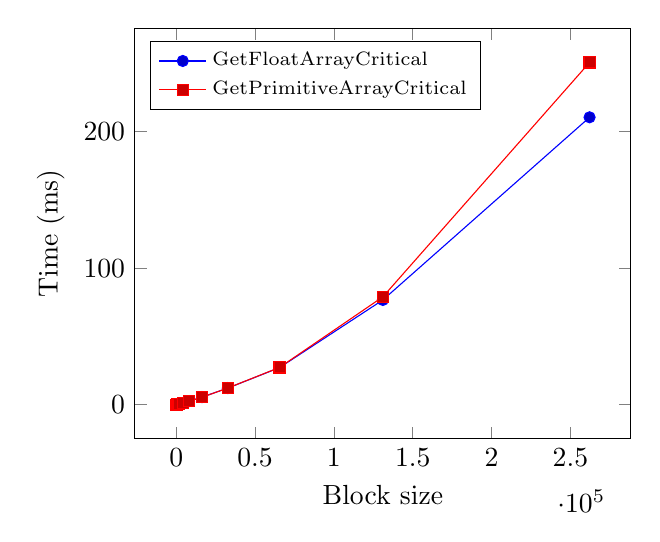
\begin{tikzpicture}
\begin{axis}[xlabel={Block size},ylabel={Time (ms)},width=0.65\linewidth,legend pos=north west,scaled y ticks = false,legend cell align=left,legend style={font=\scriptsize}]
\addplot coordinates {
(16, 0.0083)
(32, 0.0124)
(64, 0.0201)
(128, 0.0348)
(256, 0.0651)
(512, 0.1275)
(1024, 0.2659)
(2048, 0.5235)
(4096, 1.1475)
(8192, 2.6441)
(16384, 5.5785)
(32768, 12.1775)
(65536, 27.1549)
(131072, 76.6735)
(262144, 210.3414)
};
\addplot coordinates {
(16, 0.0097)
(32, 0.0132)
(64, 0.0214)
(128, 0.0342)
(256, 0.0627)
(512, 0.1225)
(1024, 0.2744)
(2048, 0.5257)
(4096, 1.1701)
(8192, 2.5845)
(16384, 5.4518)
(32768, 12.2266)
(65536, 27.2805)
(131072, 78.9501)
(262144, 250.4870)
};
\legend{GetFloatArrayCritical, GetPrimitiveArrayCritical}
\end{axis}
\end{tikzpicture}

% \end{table}
%
% \begin{table}[H]
%     \centering
%     \label{tab:cpp:princeton:recursive}
%     \caption{C++ Princeton Recursive, Time (ms)}
%     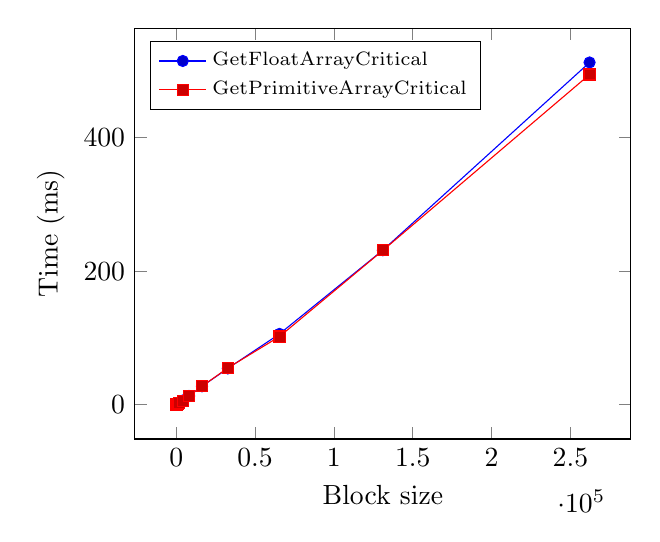
\begin{tikzpicture}
\begin{axis}[xlabel={Block size},ylabel={Time (ms)},width=0.65\linewidth,legend pos=north west,scaled y ticks = false,legend cell align=left,legend style={font=\scriptsize}]
\addplot coordinates {
(16, 0.0187)
(32, 0.0347)
(64, 0.0709)
(128, 0.1447)
(256, 0.3014)
(512, 0.6505)
(1024, 1.3689)
(2048, 2.9279)
(4096, 6.2499)
(8192, 13.1419)
(16384, 27.7314)
(32768, 54.4151)
(65536, 106.1420)
(131072, 231.5323)
(262144, 512.7674)
};
\addplot coordinates {
(16, 0.0202)
(32, 0.0368)
(64, 0.0705)
(128, 0.1434)
(256, 0.2978)
(512, 0.6379)
(1024, 1.3437)
(2048, 2.8773)
(4096, 6.1206)
(8192, 13.2345)
(16384, 27.6080)
(32768, 55.1227)
(65536, 102.1585)
(131072, 231.2663)
(262144, 494.7038)
};
\legend{GetFloatArrayCritical, GetPrimitiveArrayCritical}
\end{axis}
\end{tikzpicture}

% \end{table}
%
% \begin{table}[H]
%     \centering
%     \label{tab:cpp:columbia:iterative}
%     \caption{C++ Columbia Iterative, Time (ms)}
%     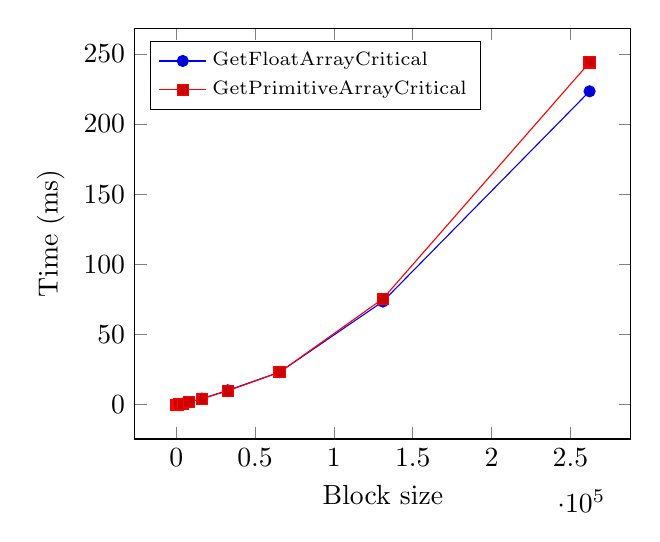
\begin{tikzpicture}
\begin{axis}[xlabel={Block size},ylabel={Time (ms)},width=0.65\linewidth,legend pos=north west,scaled y ticks = false,legend cell align=left,legend style={font=\scriptsize}]
\addplot coordinates {
(16, 0.0057)
(32, 0.0070)
(64, 0.0092)
(128, 0.0136)
(256, 0.0222)
(512, 0.0418)
(1024, 0.0970)
(2048, 0.2761)
(4096, 0.7818)
(8192, 1.8794)
(16384, 4.3304)
(32768, 10.2608)
(65536, 23.1917)
(131072, 73.5225)
(262144, 223.3088)
};
\addplot coordinates {
(16, 0.0072)
(32, 0.0086)
(64, 0.0083)
(128, 0.0115)
(256, 0.0200)
(512, 0.0366)
(1024, 0.0773)
(2048, 0.2604)
(4096, 0.7974)
(8192, 1.9326)
(16384, 4.2789)
(32768, 9.9388)
(65536, 23.1031)
(131072, 75.4942)
(262144, 243.8496)
};
\legend{GetFloatArrayCritical, GetPrimitiveArrayCritical}
\end{axis}
\end{tikzpicture}

% \end{table}
%
% \begin{table}[H]
%     \centering
%     \label{tab:cpp:kiss}
%     \caption{C++ KISS, Time (ms)}
%     /home/algo/Skola/Exjobb/Data/results/FFT/CPP_KISS_N_30.tex
% \end{table}
% \begin{table}
%     \centering
%     \label{tab:cpp:columbia:iterative:optimized}
%     \caption{C++ Columbia Iterative Optimized, Time (ms)}
%     \input{Data/results/FFT/CPP_Columbia_optimized.tex}
% \end{table}

% \begin{table}
%     \centering
%     \label{fig:java:columbia:iterative:optimized}
%     \caption{Label here}
%     \input{Data/results/FFT/Java_Columbia_optimized_Iterative.tex}
% \end{table}

% \section{Bar charts}

% \begin{figure}
%     \centering
%     \input{Data/results/FFT/Java_Princeton_Recursive_barchart.tex}
%     \label{fig:java:princeton:recursive:barchart}
%     \caption{Java Princeton Recursive bar chart}
% \end{figure}
